\documentclass{standalone}
\usepackage{tikz, xcolor, amsmath}
\begin{document}
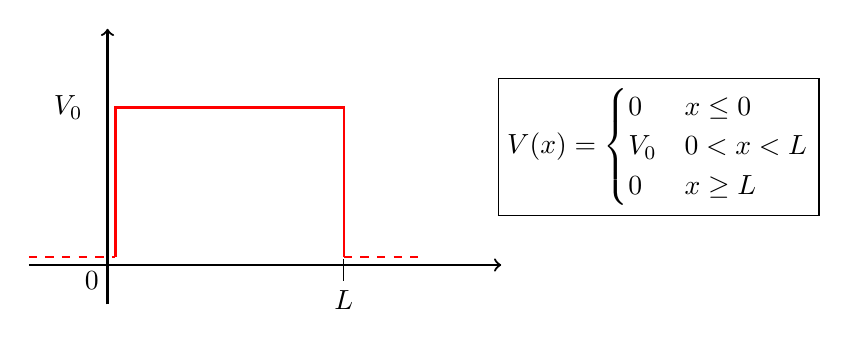
\begin{tikzpicture}
    \draw[thick, ->] (-1,0) --+ (6,0) ;
    \draw[thick, ->] (0,-0.5) --+ (0,3.5) ;
    \draw[thick, red] (0.1, 0.1) -- (0.1, 2) -- (3, 2) -- (3, 0.1) ;
    \draw[thick, red, dashed] (-1, 0.1) -- (0.1, 0.1) ;
    \draw[thick, red, dashed] (3, 0.1) -- (4, 0.1) ;
    \draw (3, 0.07) -- (3, -0.2) node[below] {$L$} ;
    \node at (-0.5, 2) {$V_0$} ;
    \node at (7, 1.5) {$\boxed{V(x) = \begin{cases}
    0 &x\leq 0 \\
    V_0 & 0 < x < L \\
    0 &x\geq L \\
    \end{cases}}$
    } ;
    \node at (-0.2, -0.2){$0$};
    
\end{tikzpicture}
\end{document}